\chapter{Astronomical calculations}

\section{Sensitivity}
\label{sec:sens-calc}
The RMS noise for multiple observations $\sigma$ is accumulated as shown in equation \ref{eq:rms-noise}.
\begin{equation}
\label{eq:rms-noise}
\sigma = \frac{\sqrt{\sum_{i=1}^M \sigma_i^2}}{M}
\end{equation}
where $M$ is the number of SBs and $\sigma_i$ is the RMS noise for a single
execution of an SB, calculated differently depending of the type of observation.
For interferometric observations the sensitivity is given by equation \ref{eq:sensitivity-interferometry}.
\begin{equation}
\label{eq:sensitivity-interferometry}
\sigma_i^{INT} = \frac{T_{sys}^i}{\eta_Q \sqrt{N_{INT}^i(N_{INT}^i-1)(\Delta\nu)\tau^i}}
\end{equation}
where $T_{sys}^i$ is the system temperature, $\eta_Q$ is the correlator sensitivity,
$N_{INT}^i$ is the number of antennas, $\Delta\nu$ is the bandwidth, and $\tau^i$ is
the integration time. All the quantities with the $i$ superscript are specific for the $i$-th
observation.

For single-dish observations
\begin{equation}
\sigma_i^{SD} = \frac{\alpha T_{sys}^i \sqrt{N_{SD}^i}}{\sqrt{(\Delta\nu)\tau^i}}
\end{equation}
where $\alpha$ is a numerical factor that depends on the scanning mode ($\sim 1$ for OTF,
$\sim \sqrt{2}$ for switched observations).

The RMS values are expressed in degrees Kelvin. To convert them to flux units, they are multiplied by the factor $2k/A_e$ where $k$ is the Boltzmann constant and $A_e$ is the antenna effective aperture.

These equations do not cover the case of the combined array, where the antennas in the array have different sizes, nor cover the cases where the bandwidth has been changed (multi-resolution modes, etc.).

\section{System Temperature}
\label{sec:tsys-calc}
The calculation of $Tsys$ is done in three steps:
\begin{enumerate}
\item First the Precipitable Water Vapor (PWV) content is determined. There are
several ways of doing this:
\begin{enumerate}
\item Calculate PWV from the Relative Humidity (RH) or the Dew Point. One way
of doing this is found in~\cite{butler98}. In this memo the PWV is developed as
$$
h = \frac{m_w P_0 H}{\rho_l k T_0}
$$
where $m_w$ is the mass of a water molecule (18 amu), $P_0$ is the water vapor
partial pressure, $H$ is the scale height of water vapor distribution (an
exponential distribution, 1.5 km for the VLA), $\rho_l$ is the density of
liquid water ($\mathrm{gr}/\mathrm{cm}^3$) and $k$ is the Boltzmann constant.

This memo presents a way to estimate $P_0$ from the dew point. In the subsequent
MMA Memo~\cite{butler98_1}, a way of calculating
$P_0$ from the relative humidity is given:
$$
P_0 = 2.409 \times 10^{12} \ RH\ \theta^4 \exp(-22.67\theta)
$$
where $\theta$ is the inverse temperature ($\theta = 300/T_0 $ K), and $RH$ is
the relative humidity.

\item Calculate it from the opacity $\tau_{225}$ at 225 GHz measured by the
tipper. In this case a way of calculating the $PWV$ can be seen in~\cite{delgado99}. $PWV$ can be obtained
by inverting
$$
\tau_{225} = 6.7787\cdot 10^{-3} + 4.0757\cdot 10^{-2} PWV + 9.59\cdot 10^{-4} PVW^2
$$
\item Get the PWV directly from the Water Vapor Radiometers.
\end{enumerate}
When the $PWV$ is available from different sources, the different values
are averaged.

\item Interpolate the ATM tables to determine the opacity $\tau$ and the
atmospheric effective temperature $T_{atm}$. The ATM tables have the following structure:
\begin{eqnarray*}
\tau & = & \tau(\nu_i, PWV_j) \\
T_{atm} & = & T_{atm}(\nu_i, PWV_j)
\end{eqnarray*}
where $\nu_i$ covers the range $20-1000$ GHz with 100 MHz granularity, and $PWV_j$
covers the 7 values 0.4772, 0.658, 0.9134, 1.262, 1.796, 2.748, and 5.186 (mm). 
\item The system temperature is calculated as:

$$
T_{sys} = \frac {\left ( T_{rx} + T_{ant} + \xi T_{ant} \right ) e^{\tau / \sin(el)}}
{\eta}
$$
where $T_{rx}$ is the receiver temperature, $\eta$ is the forward efficiency (or
feed efficiency, or spillover factor), $T_{ant}$ is the antenna temperature and $\xi$
is the sideband ratio, which for practical purposes will be $0$

Expanding the calculation of above:

$$
T_{sys} = \frac{\left ( T_{rx} + \eta T_{atm} \left ( 1 - e^{-\tau/\sin(el)} \right ) + (1 - \eta) 0.95 T_{amb} + \eta 2.76 e^{-\tau/\sin(el)} \right )  e^{\tau / \sin(el)}}
{\eta}
$$
where $T_{amb}$ is the ambient temperature, which is read from weather station.
\end{enumerate}

\section{Source visibility analysis}
\label{sec:sb-visibility}
From~\cite{meeus98} the altitude of a certain sky source is defined as shown by equation~\ref{eq:source-altitude}
\begin{equation}
\label{eq:source-altitude}
sin(h) = sin(\varphi) sin(\delta) + cos(\varphi) cos(\delta) cos(H)
\end{equation}
Where $h$ is the altitude, positive above the horizon, negative below; $\varphi$ is the observatory's latitude, positive is in northern hemisphere, negative in southern hemisphere; $\delta$ is the declination of the source, positive is north of the celestial equator, negative if south; and $H$ is the local hour angle, measured westwards from the South.

$H$ is calculated as shown by equation~\ref{eq:hour-angle-calculation}
\begin{equation}
\label{eq:hour-angle-calculation}
H = \theta - \alpha
\end{equation}
Where $\theta$ is the Local Sidereal Time (LST) and $\alpha$ is the right ascension of the sky source, usually it is expressed in terms of hours, minutes and seconds.

From these equations is possible to derive that the highest altitude in the sky is reach when $H = 0$. Or expressed in terms of LST, when $\theta = \alpha$. At this point is when there are less atmosphere between the observatory and the sky source, hence the quality of the data taken is better.

Nevertheless also it is possible to observe a sky source 
while it is not at its highest altitude in the sky, the key is to set a minimal altitude to allow to carry on observations properly. This minimum allowed altitude for ALMA observatory is set to $15^\circ$ mostly due to the surrounding mountains around the site. 

\section{Array Configuration duration and LST relationship}
\label{sec:array-visibility}
As stated in the general condition in section~\ref{sec:array-problem-general-condition} the minimum resolution for the problem is one (1) week.

From the algorithm used to calculate the LST found in~\cite{kaplan05}, it is possible to deduce that the LST drifts from the calendar time. The drift calculated rate is approximately $1654.7328\,[s]$ or $27.57888\,[min]$ ahead for every calendar week.

Therefore, the LST interval during the minimum array lifespan (of 4 weeks) will be approximately the number of hours in the daily time interval plus $1.838592\;[h]$.
Of course the borders of the configuration interval, in LST terms, would not be available the whole array duration due to the LST drifting, and these LST hours will have less representation as the array configuration life advances. But for a crude estimation of the LST interval available during array configuration life, works fine.

The minimum configuration duration set by the problem and its model definition (4 weeks), may be changed according to the total time requested by the Scheduling Blocks covered under the calculated LST range for the given array configuration. Then, the array configuration lifespan could be either the minimum duration defined by the problem, or the total time requested by the Scheduling Blocks, or a value between both.

\chapter{ALMA Project Data Model brief description}
\label{sec:apdm}
The ALMA Software system works using the concept of an Observing Project, the full description and the details of the model are available at~\cite{bridger09}. The Observing Project is used throughout the ALMA software as the top level structure associated with a project resulting from a single observing proposal. In fact the Observing Project is a container for all the information relating to a project before it begins execution. During and following execution other data associated with the project are created and held in other structures, each of which holds a reference to the original observing project. Of particular interest is the Project Status structure, which holds a record of the execution status of the Project. The ALMA Project Data Model (APDM) defines the structure of both the Observing Project (ObsProject) and the execution status (ProjectStatus).

The Scheduling Block (SchedBlock or SB) is the atomic unit of observing for ALMA, any given science observation will usually be broken into many SBs, which may, or may not be executed in sequence. The ALMA Scheduling Software will decide on which SB to execute at any given time on the basis of which is the best to execute now.

\begin{description}
\item[Observation Project Entity] \hfill \\
When a ALMA user submits a project to the Data Base, then the user is creating a ObsProject. Almost all the end-user tools in ALMA operates on ObsProjects, no other entities are exposed to the end user.

In order to hold all of the pre-observing information associated with a project the ObsProject entity class is composed of three parts: an ObsProposal, an ObsReview and an ObsProgram. These hold the information associated with the three phases of observing preparation: the proposal or Phase I; the reviewing and resultant approvals where the \textit{scientific value} is assigned by the \textit{Time Assignment Committee}; and the observing program definition, or Phase II.

\item[Observation Program Entity] \hfill \\
The Observing Program (ObsProgram) part of the Observing Project holds all the information created during Phase II, or program preparation. The ObsProgram consists of an Observing Plan (ObsPlan) and a SciencePlan. The Science Plan covers the science goal oriented view of the observing, and it is intended to contain the information that most users will use to define their observing programs. This information will persist, for the convenience of users, but will not be the definition that is used by the Observatory when carrying out the observations. Instead the latter information is contained within the ObsPlan, and covers what we call the system view. The service of Program Generation allows users to create the Observing Plan from their Science Plan. It is also possible for very advanced users to ignore the Science Plan and simply create all of the Observing Plan directly.

As stated, the Observing Plan (ObsPlan) is the container for defining the actual observing objects. In modeling terms the ObsPlan is a role for the top level ObsUnitSet, heading the definition of the system view. An ObsUnitSet contains a collection of Scheduling Blocks or more ObsUnitSets, along with objects defining the preconditions, performance and calibration requirements, and flow control that apply to that collection.


\item[Scheduling Block Entity] \hfill \\
A Scheduling Block (SB) is the unit of observing for ALMA. It defines all the information that is required by the Observatory to independently execute the acquisition of a set of data and then to calibrate it as well. Since SBs are selected for execution individually they must exist as separate items in the data base.

Most of the structures within the SB hold information that is used either by the scheduler, to query whether or not this SB is suitable for scheduling ``now'', or as information that is used by the Observing Script (in the Control subsystem) to actually execute the observing (see below), and in some cases both. There are also performance goals for the SBs, to be measured against by the observing system.

So to allow the determination of ``Schedulability'' we find items like representative target observability, weather constraints, a precondition that requires a current Baseline Calibration and a Scientific Priority.

\item[Targets] \hfill \\
The target is the element within an SB that defines the area to map, the spectral or instrumental setups to use, and the purpose of the observing. In fact the target element itself contains nothing except references to other elements that contain descriptions of these three key components.

\end{description}

\chapter{ALMA Scheduling software work-flows}
\section{DSA workflow}
\label{sec:dsa-workflow}

\begin{figure}[htbp]	
\begin{center}
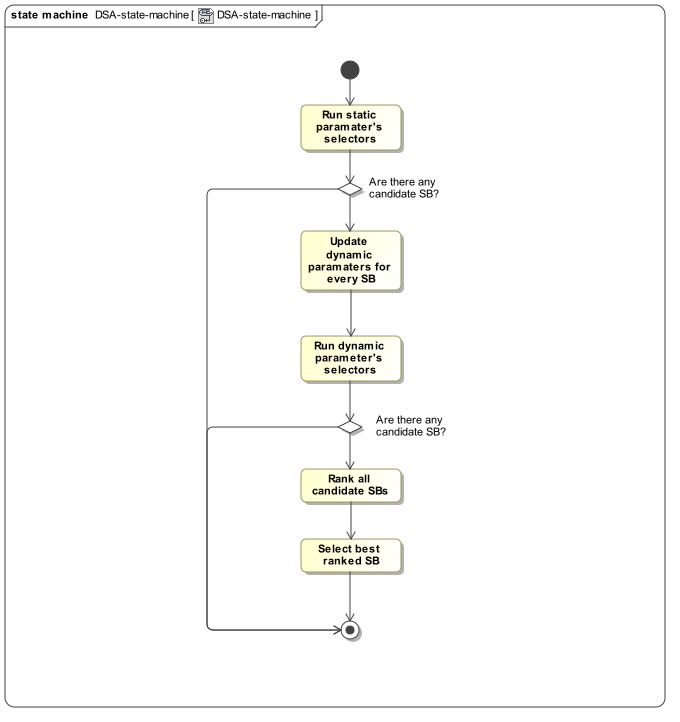
\includegraphics[width=0.9\textwidth]{images/DSA-state-machine}
\end{center}
\caption{Dynamic scheduling algorithm's state machine}
\label{fig:sched-dsa-state-machine}
\end{figure}

\begin{description}
\item[Run static parameter's selector] \hfill \\
After running these selectors the algorithm will return a list of the potential candidates given current static conditions, this includes the visibility for the representative target which is known beforehand, but is not filterable until the algorithm knows the current Local Sidereal Time. If after this state there is no feasible solution, then the algorithm will return nothing.

\item[Update dynamic parameters] \hfill \\
In this state the algorithm will recalculate the parameters requiring update at the given time. Usually weather conditions and parameters that cannot be calculated beforehand (e.g. altitude of a source for the given time, the point in the sky is in RA-Dec coordinates).  

\item[Run dynamic parameter's selector] \hfill \\
This will filter out all the Scheduling Blocks which do not fit in the criteria established after the dynamic updates ran. As the first state it will return a list of the candidate SB. If after this state there is no feasible solution, then the algorithm will return nothing.

\item[Rank all candidate Scheduling Blocks] \hfill \\
The algorithm might have a list of scorers, each one of these ``scorers'' will assign a value between ${[ 0 , 1 ]}$. The algorithm also will have a list of weights, one per scorer. The final result of each Scheduling Blocks will be sum of all the weighted scores given to this Scheduling Block for the given time to the algorithm.

\item[Select best ranked Scheduling Block] \hfill \\
The algorithm will select, and will return, the ``best'' suitable Scheduling Blocks for the given time.

\end{description}

\section{Simulator workflow}
\label{sec:sim-workflow}
The simulator is the one used in the ALMA's scheduling subsystem. At the time when this document was written it remains mostly unchanged from its original design explained in detail in~\cite{hoffstadt10}. Nevertheless some modifications were done during the development of this work, to support the simulation of several scenarios for the solution provided for the ``Array configuration planning problem''. Next a briefly description of the simulator work-flow, shown in figure~\ref{fig:sim-state-machine}, is presented:

\begin{figure}[h!]	
\begin{center}
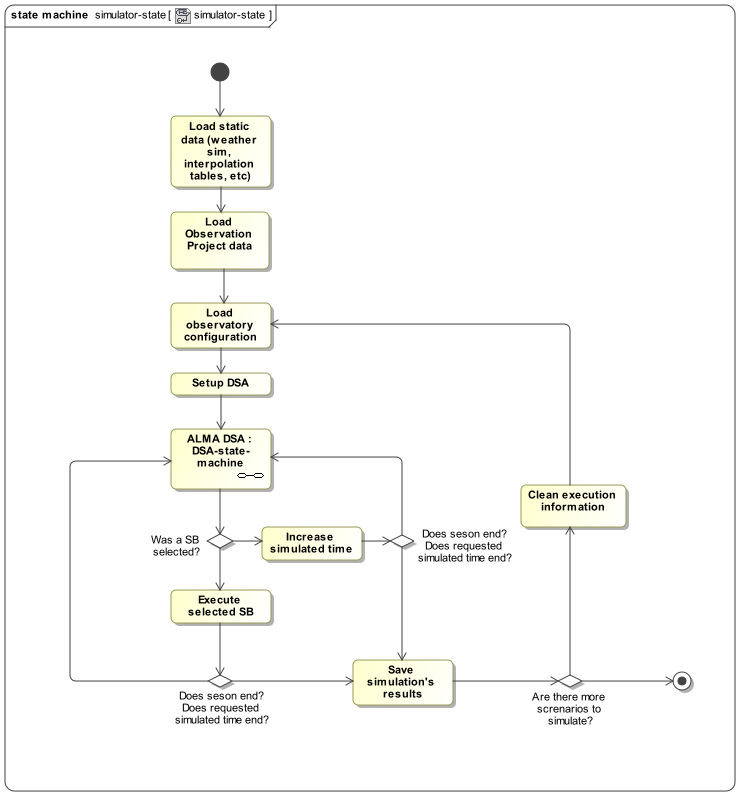
\includegraphics[width=0.67\textwidth]{images/simulator-state-machine}
\end{center}
\caption{ALMA simulator's state machine}
\label{fig:sim-state-machine}
\end{figure}

\begin{description}
\item[Load static data] \hfill \\
In this step the simulator will load all the immutable data from data-sources. This includes weather simulation data (temperature, humidity, wind speed, etc) and atmospheric interpolation tables to calculate the atmospheric opacity given the PWV and frequency. This step is separate from the rest of the data given that, the original ALMA's simulator is intended to be run using a relational database as back-end, then the data will be loaded just once.

During the development of this work, the simulator has been modified to work with data loaded completely in memory. Therefore this step add no value to the simulator itself. However it is worth of mention the difference with the original simulator used in ALMA software. 

\item[Load Observation project data] \hfill \\
In this step the simulator will load the data intended to be modified within the simulation procedure. This includes the whole observation projects, information relative to the executives and observing season.

\item[Load observatory configuration] \hfill \\
In this step the simulator loads or modifies the array configuration planning for the observing season. Originally, the ALMA's simulator supported only the loading of this data from the data-sources. During the development of this work this step was separated from the previous one, to support the setup of multiple scenarios for the, already configured, observing season.

\item[Setup DSA (algorithm for Astronomical observation scheduling problem)] \hfill \\
In this step the different simulations for each array configuration are scheduled. The simulator, according to its progress, will change among the different array configurations prepared in this step. If the simulator detects that there are no more configurations remaining for the rest of the simulated duration, then it will terminate the simulation execution and it will prepare the results and output them.

\item[Running DSA (DSA-state-machine)] \hfill \\
In this step the DSA will execute according to the work-flow presented in figure~\ref{fig:sched-dsa-state-machine} and explained in section~\ref{sec:astro-schedule-problem}.

If the DSA returns no result, then the simulator will jump $1\,[h]$ and $20\,[m]$ its simulation and try again checking whether there are selectable scheduling blocks or not. The simulator will do this until the array end time is reached.

\item[Save simulation's result] \hfill \\
After every simulation is complete, the simulator will dump a XML file containing most of the information for post-analysis.

\item[Clean execution information] \hfill \\
Since during simulation certain data for the Scheduling blocks are filled (like current number of repetitions and total time duration) and executive accounting is modified. It is necessary to clean-up all the modified data. 

The implementation done for this work will clean the complete context used for simulation, and it will reload all the data from scratch. Although it is known that this produce an overhead for the testing, it is safer to reload all the data to avoid to find programming defects during testing.
\end{description}

\chapter {Data model and implementation details}
\label{sec:implementation}
The model designed for the observation project hierarchy, is represented in figure~\ref{fig:datamodel-obsproject}, this is a simplification of the ALMA Project Data Model summarized in appendix~\ref{sec:apdm} and it is the model used in the ALMA's Dynamic Scheduling Algorithm, briefly described in section~\ref{sec:alma-dsa}.

The most relevant parts are: 
\begin{description}
\item[ObsProject] \hfill \\
This is top-level container for a group of observations requested. This container defines the scientific grade and rank, as well particular information of the executive, whom has requested the observation. All this information is shared with the set of scheduling blocks contained within.
\item[SchedBlock] \hfill \\
This is the atomic scheduling unit for the scheduling algorithm. The SB will contain information related to scheduling constraints, like array type requested, representative band, max/min angular resolution, etc; weather constraints, like, max. opacity, max. wind speed, etc; time constraints, like max. observation time, temporal boundaries; and the sky source.
\end{description}

\begin{figure}[htbp]	
\begin{center}
\includegraphics[width=1.15\textwidth]{images/Obsproject}
\end{center}
\caption{Observation Project data model}
\label{fig:datamodel-obsproject}
\end{figure}

The model designed to handle the observatory instrumentation is represented in figure~\ref{fig:datamodel-observatory}. This is an over simplification of what is presented in~\cite{avarias11, hoffstadt10}, the \textbf{ArrayConfiguration} class covers the minimal needs to allow to the algorithm to take a decision regarding the array configuration parameters. The simplification was done because the original classes defined did not add any extra value for the algorithm.

\begin{figure}[htbp]	
\begin{center}
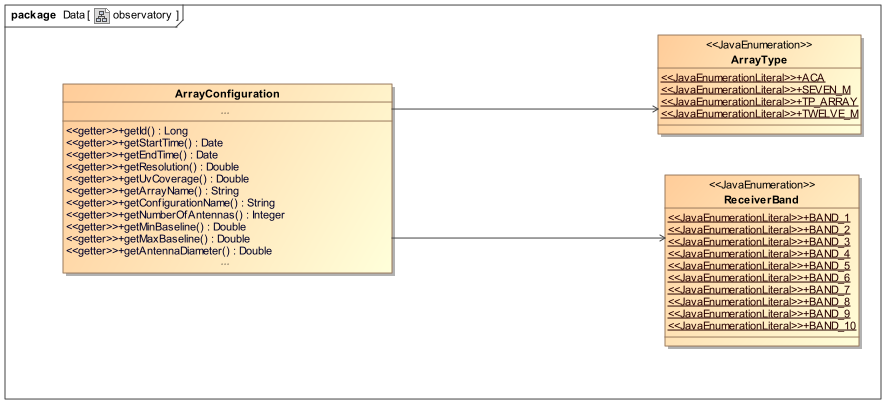
\includegraphics[width=0.67\textwidth]{images/Observatory}
\end{center}
\caption{Observatory instrumentation data model}
\label{fig:datamodel-observatory}
\end{figure}

The model designed for handle the Executive information and the observing season is represented in figure~\ref{fig:datamodel-executive}
The most relevant parts are: 
\begin{description}
\item[Executive] This class holds the information related to each executive provided as input. It saves the percentage and associates each Principal Investigator (class \textbf{PI}). Originally, the model was designed to allow to every PI have assigned percentages to each executive. However in practice, this has not been used.

\item[Observing Season] This class has the information related to the start and end dates for the observing season or observing cycle, also keeps the information relative to the daily schedule, in a \textbf{TimeInterval} class instance.
\end{description}

\begin{figure}[htbp]	
\begin{center}
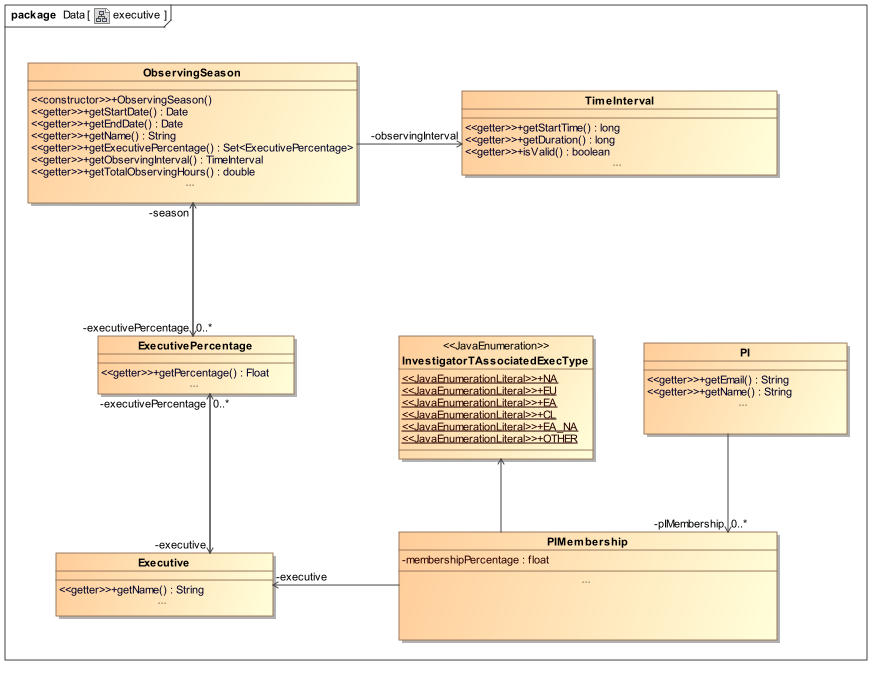
\includegraphics[width=0.67\textwidth]{images/Executive}
\end{center}
\caption{Executive and observing season data model}
\label{fig:datamodel-executive}
\end{figure}

The model designed to handle the weather is represented in figure~\ref{fig:datamodel-weather}. The weather model is quite simple, it has several classes holding data for the simulated weather, like precipitable water vapor, temperature, wind speed and phase. Also the model has the class \textbf{AtmParamters}, which contains the interpolation tables to calculate the atmospheric opacity.

\begin{figure}[htbp]	
\begin{center}
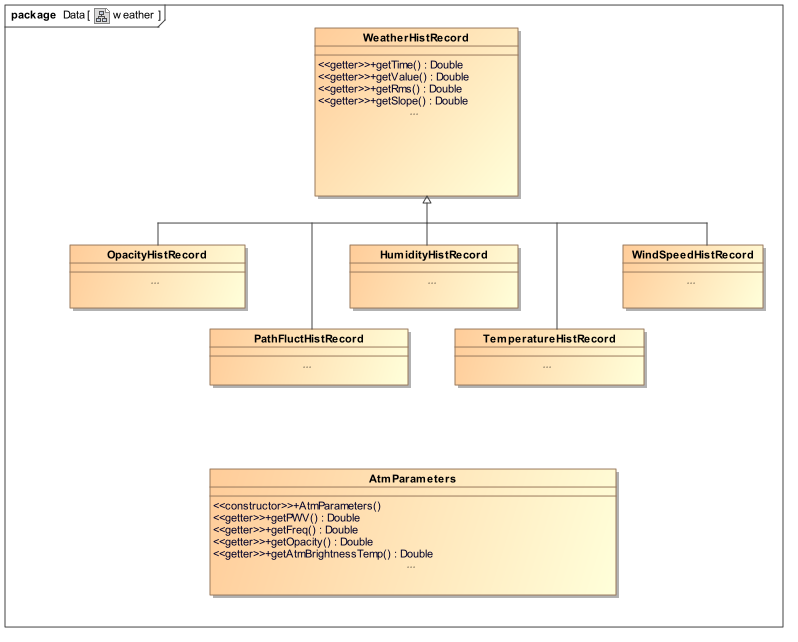
\includegraphics[width=0.67\textwidth]{images/Weather}
\end{center}
\caption{Weather data model}
\label{fig:datamodel-weather}
\end{figure}

The model designed to handle the observation progress status is represented in figure~\ref{fig:datamodel-observation}. This model defines the \textbf{ExecBlock}, which keeps the time accounting and progress for each SB, array configuration and Executive. 

\begin{figure}[htbp]	
\begin{center}
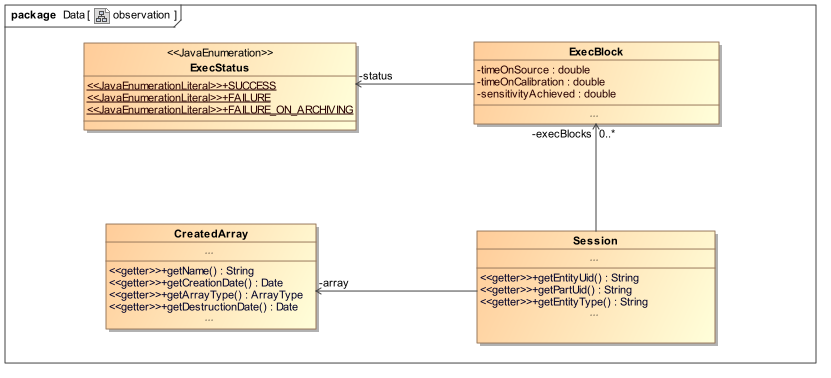
\includegraphics[width=0.67\textwidth]{images/Observation}
\end{center}
\caption{Observation progress status}
\label{fig:datamodel-observation}
\end{figure}

The top-level architecture of the ALMA's scheduling planning simulator is represented in diagram~\ref{fig:sim-top-level-architecture}. The software design uses as glue the Spring Core library, using Inversion of Control paradigm is possible to define via a configuration file, the objects to inject into the simulator, this includes Data Access Objects instances and the algorithm instances. It is enough for the software developed in this work to implement the correct interfaces to make them compatible with the rest of the ALMA software.

For the development of the validation software prepared for this work, some changes were done. Essentially the whole DAO's code, presented in the left part and on bottom part of the figure~\ref{fig:sim-top-level-architecture}, which is particular to ALMA software, were replaced with a Data Accessors able to read the XML format defined by the scheduling subsystem software, for data-interchange; and with in-memory data structures provided by the Java API, respectively. The core of the simulator tool and the algorithm does not deal directly with the data, instead a Data Accessors Object (DAO) interface was defined already by the ALMA's scheduling software, which abstracts all the interaction between the simulator and the data. Hence the replacement was fairly easy.

\begin{figure}[h!]	
\begin{center}
\includegraphics[width=0.67\textwidth]{images/simulator-arch}
\end{center}
\caption{Current top-level ALMA's scheduling simulator tool}
\label{fig:sim-top-level-architecture}
\end{figure}

In other hand, the algorithm implemented by ALMA software (DSA) was replaced with the modified Deficit Round-Robin algorithm implementation presented in this work (see chapter~\ref{sec:astro-schedule-problem}). The ALMA software design also make provisions at the algorithm level, defining an interface, which, as well as the DAOs, was fairly easy to replace with new classes developed to implement the modified DRR algorithm.

\chapter{Scheduling Block critical subset for each array configuration}
\label{sec:sb-critical-set}
\begin{figure}[htbp]
        \centering
        \begin{subfigure}[b]{0.45\textwidth}
                \includegraphics[width=\textwidth]{images/c34-1_sources}
                \caption{C34-1} 
        \end{subfigure} 
        ~ %
%
        \begin{subfigure}[b]{0.45\textwidth}
                \includegraphics[width=\textwidth]{images/c34-2_sources}
                \caption{C34-2}
        \end{subfigure}

        \begin{subfigure}[b]{0.45\textwidth}
                \includegraphics[width=\textwidth]{images/c34-3_sources}
                \caption{C34-3}
        \end{subfigure}
        ~ 
        \begin{subfigure}[b]{0.45\textwidth}
                \includegraphics[width=\textwidth]{images/c34-4_sources}
                \caption{C34-4}
        \end{subfigure}% 
        
        \begin{subfigure}[b]{0.45\textwidth}
                \includegraphics[width=\textwidth]{images/c34-5_sources}
                \caption{C34-5}
        \end{subfigure}
        ~
        \begin{subfigure}[b]{0.45\textwidth}
                \includegraphics[width=\textwidth]{images/c34-6_sources}
                \caption{C34-6}
        \end{subfigure}
        
        \begin{subfigure}[b]{0.45\textwidth}
                \includegraphics[width=\textwidth]{images/c34-7_sources}
                \caption{C34-7}
        \end{subfigure}           
        \caption{Visibility of A-graded Scheduling Blocks for $12\,[m]$ Array Configurations}
		\label{fig:results-sb-critical-set}
\end{figure}

The LST intervals proposed by the Scheduling Block classification software can be seen in table~\ref{table:lst-int-prop}.

\begin{table}[htbp]
\begin{center}
\begin{tabular}{|c|c|c|}
\hline
\textbf{Array configuration} & \textbf{Start time (LST)} & \textbf{End time (LST)} \\ \hline
C34-1 & 5.61692 & 15.45551 \\ \hline
C34-1 & 13.30675 & 23.14534 \\ \hline
C34-2 & 9.86519 & 19.703777 \\ \hline
C34-2 & 13.22811 & 23.06670 \\ \hline
C34-3 & 4.44851 & 14.28710 \\ \hline
C34-3 & 9.76941 & 19.60800 \\ \hline
C34-3 & 12.97411 & 22.81270 \\ \hline
C34-4 & 5.61692 & 15.45551 \\ \hline
C34-5 & 9.93925 & 19.77784 \\ \hline
C34-6 & 21.92851 & 7.76710 \\ \hline
C34-7 & 2.77808 & 12.61667 \\ \hline
C34-7 & 4.94547 & 14.78406 \\ \hline
C34-7 & 9.76941 & 19.60800 \\ \hline
\end{tabular}
\end{center}
\caption[LST intervals proposed by the Scheduling Blocks categorization]
{LST intervals proposed by the Scheduling blocks categorization described in section~\ref{sec:array-sb-classification}}
\label{table:lst-int-prop}
\end{table}

Comparing both, the sources elevation vs LST intervals proposed by the algorithm, it is possible to see that most of A-graded SB's sky sources are covered on those proposed LST intervals.
